%%%%%%%%%%%%%%%%%%%%%%%%%%%%%%%%%%%%%%%%%%%%%%%%%%%%%%%%%%%%%%%%%%%%%%
% How to use writeLaTeX: 
%
% You edit the source code here on the left, and the preview on the
% right shows you the result within a few seconds.
%
% Bookmark this page and share the URL with your co-authors. They can
% edit at the same time!
%
% You can upload figures, bibliographies, custom classes and
% styles using the files menu.
%
%%%%%%%%%%%%%%%%%%%%%%%%%%%%%%%%%%%%%%%%%%%%%%%%%%%%%%%%%%%%%%%%%%%%%%

\documentclass[12pt]{article}

\usepackage{sbc-template}

\usepackage{graphicx,url}

%\usepackage[brazil]{babel}   
\usepackage[utf8]{inputenc}  
\graphicspath{ {./imgs/} }
     
\sloppy

\title{Apresentação de Jogo Interativo\\Baseado em Heatmap}

\author{Draylon Lopes\inst{1}, Felipe Goularte\inst{2}, Gustavo Michels de Camargo\inst{3}, Victor Bernardes\inst{4} }


\address{Departamento de Ciência da Computação -- Universidade do Estado de Santa Catarina (UDESC)\\
  Joinville-- SC -- Brazil
}

\begin{document} 

\maketitle

\begin{abstract}
  This meta-article aims to present the results of the interactive game that took place in the classroom during Human–computer interaction classes.
\end{abstract}
     
\begin{resumo} 
  Este meta-artigo tem como objetivo apresentar os resultados do jogo interativo que decorreu em sala durante as aulas de Interação Homem Computador.
\end{resumo}

\section{Introdução}

Como ultima avaliação da diciplina de Interação Homem Computador, foi requerido uma pequena implementação de um jogo interativo para propositos de estudo para cada equipe sobre os temas distribuidos pela professora e orientadora Isabela Gasparini, este jogo e ocasional pesquisa subsequente vem como parte da parte 2 das discuções entre os temas distribuidos entre as equipes.

Nossa equipe ficou a cargo dos conceitos e aplicações de Heatmap e relacioados, que anteriormente apresentamos em sala de aula para os demais estudantes e para a professora.


\section{O Jogo}

O grupo inicialmente apresentou novamente e resumidamente o que é Heatmap e seus diversos tipos existentesm, seria necessario para que os jogadores pudessem realizar a atividade proposta com melhor clareza, em seguida eles deveriam entrar na plataforma online Kahoot para que se desse início ao jogo interativo.

Com o jogo em andamento era exibido para os jogadores diversas questões individuais com imagens de diferentes tipos e estilos de heatmap e o objetivo relaciona los com o mapa de calor correto, eram questões de multipla escolha. Entre cada questão havia um tempo razoavel disponivel para que os jogares pudessem pensar, discutir e julgar a resposta correta referente a cada questão.

Ao final ficava disponivel ao jogador um relatorio com relação aos acertos e erros durante o jogo.

\section{Avaliação de usabilidade}

Após o jogo foi disponibilizado para acesso entre os jogares um formulario com perguntas sobre o jogo com possibilidade numerica de respota entre 1 e 5 para "Discordo totalmente" e "Concordo totalmente".

\section{Resultado}

Segue abaixo a lista de perguntas com o anexo de graficos de setores representando a distribuição de respostas em cada pergunta.

\subsection{O design do jogo é atraente.}

\begin{center}
  \includegraphics[scale=0.4]{O design do jogo é atraente..png}
\end{center}

\subsection{O jogo contribuiu para a minha aprendizagem na disciplina.}

\begin{center}
  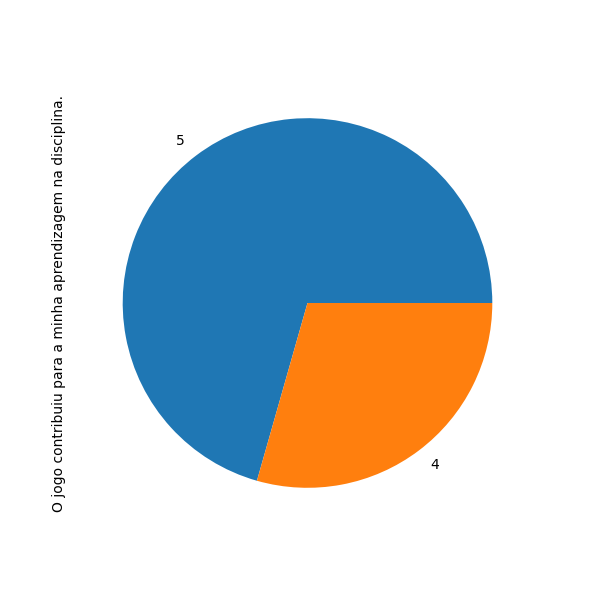
\includegraphics[scale=0.4]{O jogo contribuiu para a minha aprendizagem na disciplina..png}
\end{center}


\subsection{O jogo evolui num ritmo adequado e não fica monótono — oferece novos obstáculos, situações ou variações de atividades.}

\begin{center}
  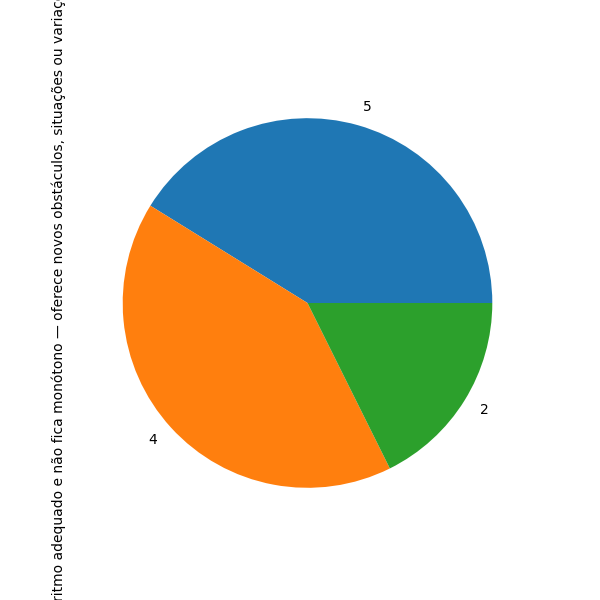
\includegraphics[scale=0.4]{O jogo evolui num ritmo adequado e não fica monótono — oferece novos obstáculos, situações ou variações de atividades..png}
\end{center}


\subsection{O conteúdo do jogo está conectado com outros conhecimentos que eu já possuía.}

\begin{center}
  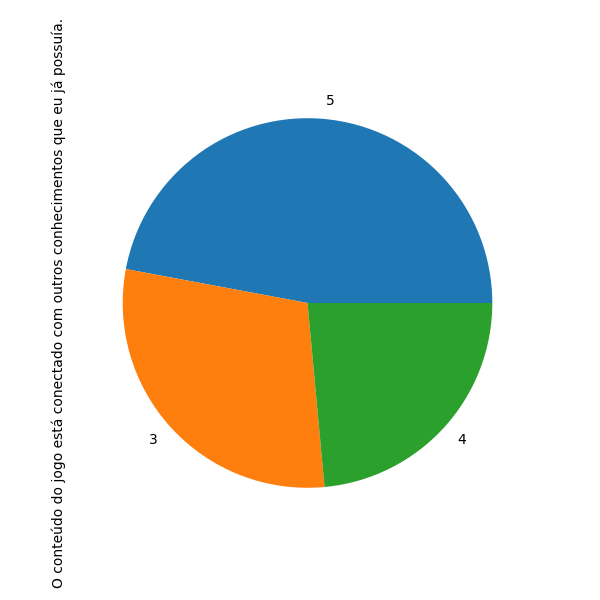
\includegraphics[scale=0.4]{O conteúdo do jogo está conectado com outros conhecimentos que eu já possuía..png}
\end{center}

\subsection{O jogo forneceu feedback constante dos meus acertos e erros durante e ao final.}

\begin{center}
  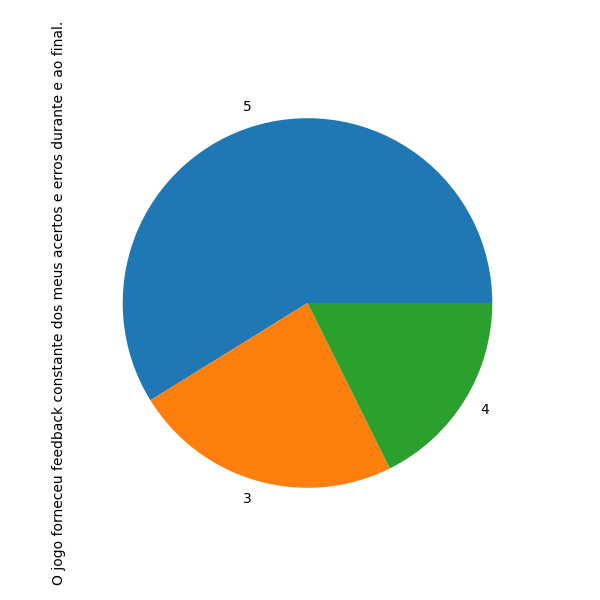
\includegraphics[scale=0.4]{O jogo forneceu feedback constante dos meus acertos e erros durante e ao final..png}
\end{center}

\subsection{Eu gostei do jogo e não me senti ansioso ou entediado por causa dele.}

\begin{center}
  \includegraphics[scale=0.4]{Eu gostei do jogo e não me senti ansioso ou entediado por causa dele..png}
\end{center}

\subsection{A organização das informações na tela está clara e objetiva}

\begin{center}
  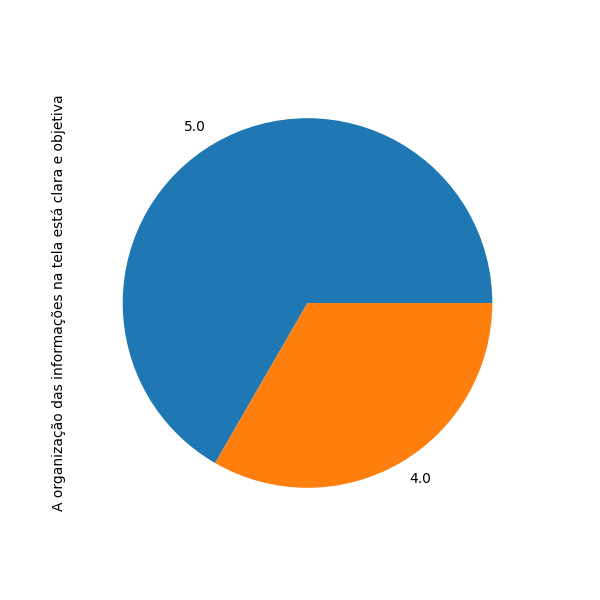
\includegraphics[scale=0.4]{A organização das informações na tela está clara e objetiva.png}
\end{center}

\subsection{Esquema de pontuação de acertos e erros foi feita de forma justa}

\begin{center}
  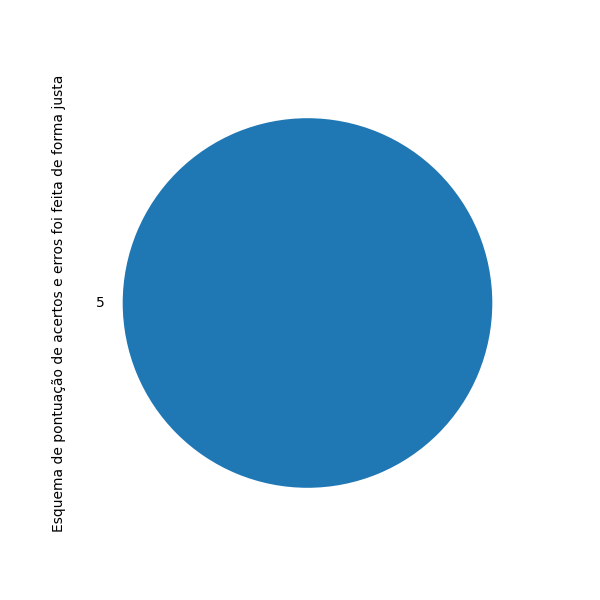
\includegraphics[scale=0.4]{Esquema de pontuação de acertos e erros foi feita de forma justa.png}
\end{center}

\subsection{Foi fácil entender o jogo.}

\begin{center}
  \includegraphics[scale=0.4]{Foi fácil entender o jogo..png}
\end{center}

\subsection{O tempo de jogo foi satisfatório.}

\begin{center}
  \includegraphics[scale=0.4]{O tempo de jogo foi satisfatório..png}
\end{center}


\section{Conclusão}

Na maioria das perguntas os jogadores avaliaram o jogo interativo de forma satisfatoria, com restrita exceção sobre a satisfação ao tempo de jogo em que uma pequena porcentagem dos jogadores discordou e haveria de procurar descobrir qual a razão por trás disso, se é por falta de tempo ou algo relacionado.

\bibliographystyle{sbc}
\bibliography{sbc-template}

\end{document}
